\PassOptionsToPackage{unicode=true}{hyperref} % options for packages loaded elsewhere
\PassOptionsToPackage{hyphens}{url}
%
\documentclass[]{article}
\usepackage{lmodern}
\usepackage{amssymb,amsmath}
\usepackage{ifxetex,ifluatex}
\usepackage{fixltx2e} % provides \textsubscript
\ifnum 0\ifxetex 1\fi\ifluatex 1\fi=0 % if pdftex
  \usepackage[T1]{fontenc}
  \usepackage[utf8]{inputenc}
  \usepackage{textcomp} % provides euro and other symbols
\else % if luatex or xelatex
  \usepackage{unicode-math}
  \defaultfontfeatures{Ligatures=TeX,Scale=MatchLowercase}
\fi
% use upquote if available, for straight quotes in verbatim environments
\IfFileExists{upquote.sty}{\usepackage{upquote}}{}
% use microtype if available
\IfFileExists{microtype.sty}{%
\usepackage[]{microtype}
\UseMicrotypeSet[protrusion]{basicmath} % disable protrusion for tt fonts
}{}
\IfFileExists{parskip.sty}{%
\usepackage{parskip}
}{% else
\setlength{\parindent}{0pt}
\setlength{\parskip}{6pt plus 2pt minus 1pt}
}
\usepackage{hyperref}
\hypersetup{
            pdfborder={0 0 0},
            breaklinks=true}
\urlstyle{same}  % don't use monospace font for urls
\usepackage[margin=1in]{geometry}
\usepackage{graphicx,grffile}
\makeatletter
\def\maxwidth{\ifdim\Gin@nat@width>\linewidth\linewidth\else\Gin@nat@width\fi}
\def\maxheight{\ifdim\Gin@nat@height>\textheight\textheight\else\Gin@nat@height\fi}
\makeatother
% Scale images if necessary, so that they will not overflow the page
% margins by default, and it is still possible to overwrite the defaults
% using explicit options in \includegraphics[width, height, ...]{}
\setkeys{Gin}{width=\maxwidth,height=\maxheight,keepaspectratio}
\setlength{\emergencystretch}{3em}  % prevent overfull lines
\providecommand{\tightlist}{%
  \setlength{\itemsep}{0pt}\setlength{\parskip}{0pt}}
\setcounter{secnumdepth}{0}
% Redefines (sub)paragraphs to behave more like sections
\ifx\paragraph\undefined\else
\let\oldparagraph\paragraph
\renewcommand{\paragraph}[1]{\oldparagraph{#1}\mbox{}}
\fi
\ifx\subparagraph\undefined\else
\let\oldsubparagraph\subparagraph
\renewcommand{\subparagraph}[1]{\oldsubparagraph{#1}\mbox{}}
\fi

% set default figure placement to htbp
\makeatletter
\def\fps@figure{htbp}
\makeatother

\usepackage{ctex}
\usepackage{xcolor}
\usepackage{fancyhdr}
\usepackage{sectsty}
\definecolor{glaucous}{rgb}{0.38, 0.51, 0.71}
\definecolor{lavenderblush}{rgb}{1.0, 0.94, 0.96}
\usepackage{enumitem}% http://ctan.org/pkg/enumitem
\usepackage[empty]{fullpage}% http://ctan.org/pkg/fullpage
\usepackage{color}% http://ctan.org/pkg/color
\usepackage{hyperref}% http://ctan.org/pkg/hyperref
\usepackage{geometry}
\geometry{a4paper,scale=0.8}
\usepackage{blindtext}
\usepackage{caption}
\usepackage{subfigure}
\usepackage{float}
\usepackage{graphicx}
\usepackage{booktabs}
\usepackage[justification=centering]{caption}
\usepackage{threeparttable}
\usepackage{booktabs}
\usepackage{longtable}
\usepackage{array}
\usepackage{multirow}
\usepackage{wrapfig}
\usepackage{float}
\usepackage{colortbl}
\usepackage{pdflscape}
\usepackage{tabu}
\usepackage{threeparttable}
\usepackage{threeparttablex}
\usepackage[normalem]{ulem}
\usepackage{makecell}
\usepackage{xcolor}
\textwidth 6.75in
\textheight 8.5in
\oddsidemargin -.25in
\evensidemargin -.25in
\topmargin -0.5in
\linespread{1.0}
\setlength{\parskip}{0.8em}
\usepackage{booktabs}
\usepackage{longtable}
\usepackage{array}
\usepackage{multirow}
\usepackage{wrapfig}
\usepackage{float}
\usepackage{colortbl}
\usepackage{pdflscape}
\usepackage{tabu}
\usepackage{threeparttable}
\usepackage{threeparttablex}
\usepackage[normalem]{ulem}
\usepackage{makecell}
\usepackage{xcolor}

\title{\textcolor{glaucous}{\Huge \textbf {新冠早报}}}
\author{\textcolor{glaucous}{\Large 第六期 3月28日}}
\date{}

\begin{document}
\maketitle

\fontsize{13}{13}
\selectfont

\newcommand{\resheading}[1]{%
  \noindent\fcolorbox{lavenderblush}{lavenderblush}{\makebox[\dimexpr\textwidth-2\fboxsep-2\fboxrule][l]{\textbf{~#1}}}%
}

\pagestyle{fancyplain}
\lhead{
\includegraphics[height=2cm]{./input/logo.png}}
\rhead{
\begin{tabular}{ccc}
\textcolor{gray}{中美健康峰会「智援组」新冠早报组}\\
\\ \\ \\ \\ \\
\end{tabular}}

\renewcommand{\headrulewidth}{0pt}
\setlength{\headheight}{50pt}

%
  \noindent\fcolorbox{lavenderblush}{lavenderblush}{\makebox[\dimexpr\textwidth-2\fboxsep-2\fboxrule][l]{\textbf{~\Large 每日新闻}}}%

\hypertarget{section}{%
\subsection{\texorpdfstring{\textcolor{glaucous}{\Large 国际}}{}}\label{section}}

\textbf{\textcolor{glaucous}{有线电视新闻网(CNN)}}:
\textbf{特朗普签署2万亿美元的经济援助法案}

当地时间3月27日下午4时30分,美国总统特朗普发推文称他签署了美国有史以来金额最大的经济援助法
案(CARES法),该法案总救济金额为2.2万亿美元,将为美国的家庭、工人和企业提供紧急救援。

\textbf{\textcolor{glaucous}{有线电视新闻网(CNN)}} :
\textbf{特朗普签署2万亿美元的经济援助法案}

当地时间3月27日下午4时30分,美国总统特朗普发推文称他签署了美国有史以来金额最大的经济援助法
案(CARES法),该法案总救济金额为2.2万亿美元,将为美国的家庭、工人和企业提供紧急救援。

\hypertarget{section-1}{%
\subsection{\texorpdfstring{\textcolor{glaucous}{\Large 国内}}{}}\label{section-1}}

\textbf{\textcolor{glaucous}{有线电视新闻网(CNN)}}:
\textbf{特朗普签署2万亿美元的经济援助法案}

当地时间3月27日下午4时30分,美国总统特朗普发推文称他签署了美国有史以来金额最大的经济援助法
案(CARES法),该法案总救济金额为2.2万亿美元,将为美国的家庭、工人和企业提供紧急救援。

\newpage

%
  \noindent\fcolorbox{lavenderblush}{lavenderblush}{\makebox[\dimexpr\textwidth-2\fboxsep-2\fboxrule][l]{\textbf{~\Large 疫情观察}}}%

数据源:约翰霍普金斯大学,The COVID Tracking Project

数据截止至:北京时间3月28日 早4:00

\hypertarget{section-2}{%
\section{\texorpdfstring{\textcolor{glaucous}{一、世界疫情}}{}}\label{section-2}}

截止北京时间3月28日早6:00,全球累计591,802例确诊病例。

\begin{figure}[H] 
\centering
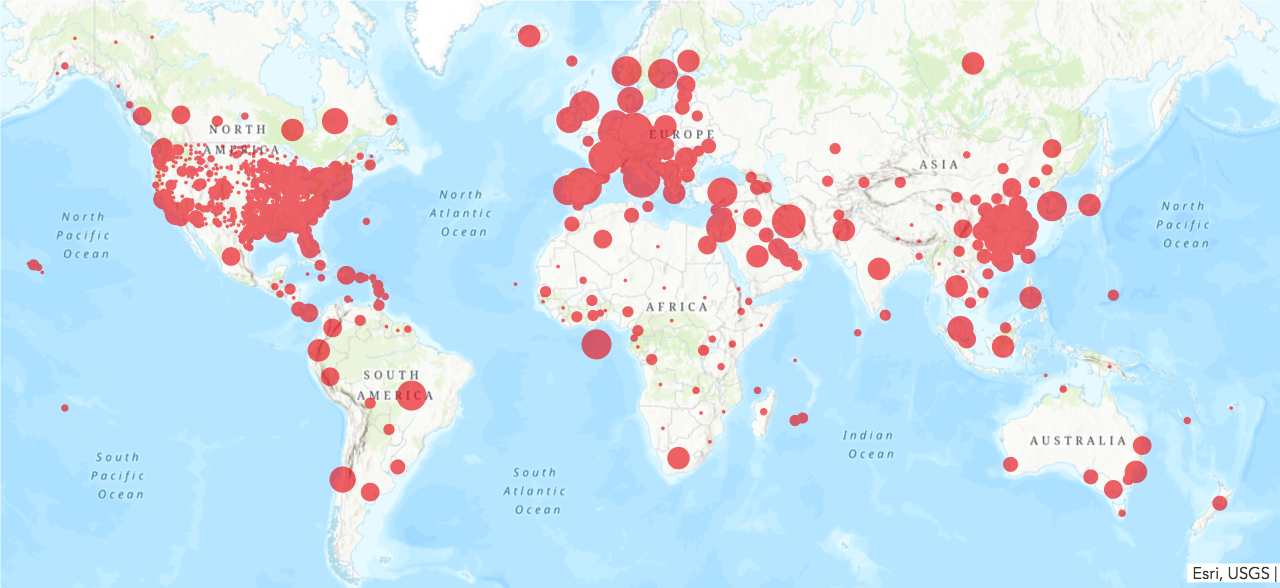
\includegraphics[]{./input/table_plot/covid1.png} %插入图片,[]中设置图片大小,{}中是图片文件名
\caption{世界疫情分布图 (Global Map of Cumulative Confirmed COVID-19 Cases)} %最终文档中希望显示的图片标题
\label{} %用于文内引用的标签
\end{figure}

\begin{table}[!htb]
    \caption{确诊前十位国家}
      \centering \begin{table}[H]
\centering
\begin{tabular}{rlrr}
\toprule
  & 国家(地区) & 累计确诊病例 & 粗发病率\\
\midrule
\rowcolor{gray!6}  1 & Hubei & 67802 & 115\\
2 & US & 213372 & 64\\
\rowcolor{gray!6}  3 & Italy & 110574 & 183\\
4 & Spain & 104118 & 223\\
\rowcolor{gray!6}  5 & China & 82361 & 6\\
\addlinespace
6 & Germany & 77872 & 93\\
\rowcolor{gray!6}  7 & France & 57749 & 88\\
8 & Iran & 47593 & 57\\
\rowcolor{gray!6}  9 & United Kingdom & 29865 & 44\\
10 & Switzerland & 17768 & 205\\
\bottomrule
\end{tabular}
\end{table} \begin{tablenotes}
        \setfontsize\footnotesize\ixpt{9}
        \item 注:粗发病率定义:累计确诊病例/10万人。计算方式:累计确诊病例/⼈×10万  %此处加入注释信息
      \end{tablenotes}
    \end{table}

\}

\begin{table}[!htb]
    \begin{minipage}{.4\linewidth}
    \caption{确诊前十位国家}
      \centering \begin{table}[H]
\centering
\begin{tabular}{rlr}
\toprule
  & 国家 & 当⽇新增病例\\
\midrule
\rowcolor{gray!6}  1 & US & 213372\\
2 & Italy & 110574\\
\rowcolor{gray!6}  3 & Spain & 104118\\
4 & China & 82361\\
\rowcolor{gray!6}  5 & Germany & 77872\\
\addlinespace
6 & France & 57749\\
\rowcolor{gray!6}  7 & Iran & 47593\\
8 & United Kingdom & 29865\\
\rowcolor{gray!6}  9 & Switzerland & 17768\\
10 & Turkey & 15679\\
\bottomrule
\end{tabular}
\end{table} \end{minipage}%
    \begin{minipage}{.4\linewidth}
    \caption{累计死亡前十位国家}
      \centering \begin{table}[H]
\centering
\begin{tabular}{rlrrr}
\toprule
  & 国家 & 累计死亡病例 & 较昨⽇ & 病死率\%\\
\midrule
\rowcolor{gray!6}  1 & Italy & 13155 & 727 & 11.9\\
2 & Spain & 9387 & 923 & 9.0\\
\rowcolor{gray!6}  3 & US & 4757 & 884 & 2.2\\
4 & France & 4043 & 511 & 7.0\\
\rowcolor{gray!6}  5 & China & 3316 & 7 & 4.0\\
\addlinespace
6 & Iran & 3036 & 138 & 6.4\\
\rowcolor{gray!6}  7 & United Kingdom & 2357 & 564 & 7.9\\
8 & Netherlands & 1175 & 135 & 8.6\\
\rowcolor{gray!6}  9 & Germany & 920 & 145 & 1.2\\
10 & Belgium & 828 & 123 & 5.9\\
\bottomrule
\end{tabular}
\end{table} \end{minipage} 
\end{table}

\}

\begin{figure}[H]
    \begin{minipage}[H]{0.5\linewidth}
    \centering
    \begin{threeparttable}
        \begin{tabular}{@{}llll@{}}
        \toprule
           & 国家(地区)         & 累计确诊病例 & 粗发病率 \\ \midrule
        1  & Hubei          & 67802  & 115  \\
        2  & US             & 213372 & 64   \\
        3  & Italy          & 110574 & 183  \\
        4  & Spain          & 104118 & 223  \\
        5  & China          & 82361  & 6    \\
        6  & Germany        & 77872  & 93   \\
        7  & France         & 57749  & 88   \\
        8  & Iran           & 47593  & 57   \\
        9  & United Kingdom & 29865  & 44   \\
        10 & Switzerland    & 17768  & 205  \\ \bottomrule
        \end{tabular}
        \begin{tablenotes}
        \footnotesize
        \item[*] 粗发病率定义:累计确诊病例/10万人。计算方式:累计确诊病例/⼈×10万  %此处加入注释信息
      \end{tablenotes}
    \end{threeparttable}
        \makeatletter\def\@captype{table}\makeatother\caption{确诊前十位国家\\ \ }
    \end{minipage}%
    \begin{minipage}[H]{0.5\linewidth}
    \centering
    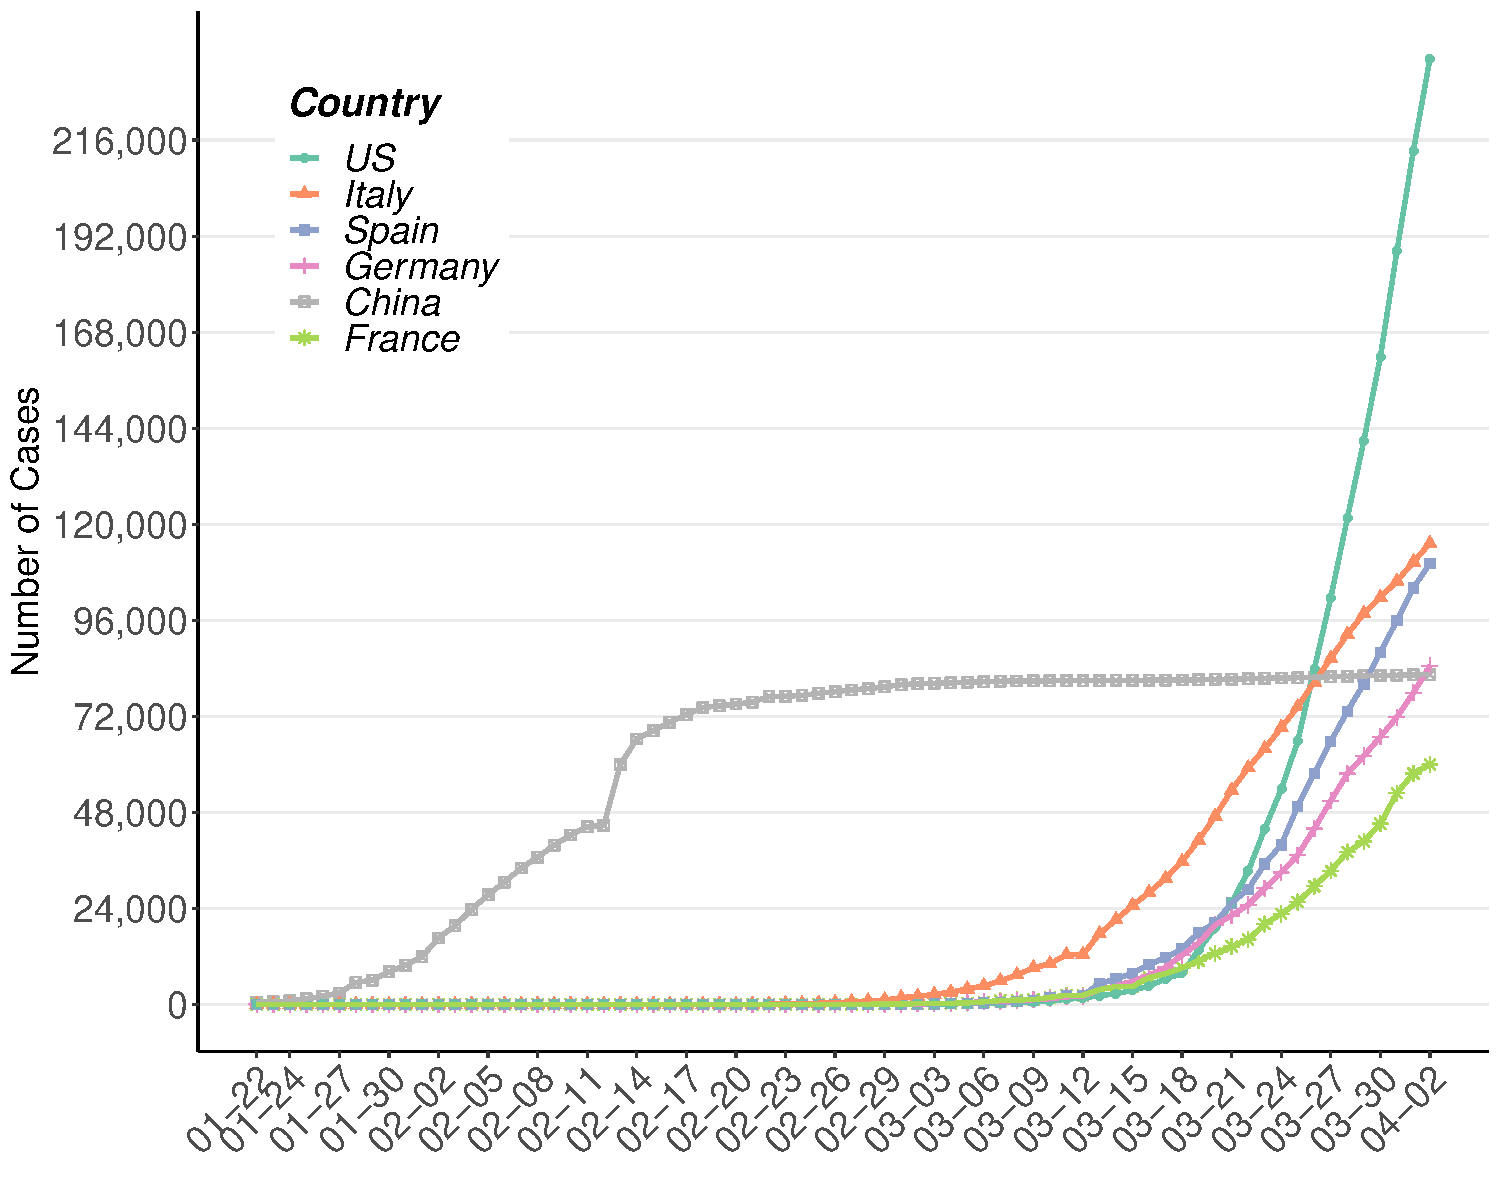
\includegraphics[]{./input/table_plot/covid2.pdf}
    \caption{累计确诊病例国家趋势图\\(中国及其他前五位国家)}
    \end{minipage}
\end{figure}

从累计死亡病例数(表2)来看,全球累计死亡病例数前十国家位次不变。

\begin{minipage}{\textwidth}\small
        \begin{minipage}[H]{0.3\textwidth}
        \centering
           \begin{tabular}{@{}lll@{}}
            \toprule
               & 国家             & 当日新增病例 \\ \midrule
            1  & US             & 213372 \\
            2  & Italy          & 110574 \\
            3  & Spain          & 104118 \\
            4  & China          & 82361  \\
            5  & Germany        & 77872  \\
            6  & France         & 57749  \\
            7  & Iran           & 47593  \\
            8  & United Kingdom & 29865  \\
            9  & Switzerland    & 17768  \\
            10 & Turkey         & 15679  \\ \bottomrule
            \end{tabular}
            \makeatletter\def\@captype{table}\makeatother\caption{日新增病例前十位国家}
        \end{minipage}
        \begin{minipage}[H]{0.65\textwidth}
        \centering
           \begin{tabular}{@{}lllll@{}}
          \toprule
             & 国家             & 累计死亡病例 & 较昨⽇ & 病死率\% \\           \midrule
          1  & Italy          & 13155  & 727 & 11.9  \\
          2  & Spain          & 9387   & 923 & 9     \\
          3  & US             & 4757   & 884 & 2.2   \\
          4  & France         & 4043   & 511 & 7     \\
          5  & China          & 3316   & 7   & 4     \\
          6  & Iran           & 3036   & 138 & 6.4   \\
          7  & United Kingdom & 2357   & 564 & 7.9   \\
          8  & Netherlands    & 1175   & 135 & 8.6   \\
          9  & Germany        & 920    & 145 & 1.2   \\
          10 & Belgium        & 828    & 123 & 5.9   \\ \bottomrule
          \end{tabular}
      \makeatletter\def\@captype{table}\makeatother\caption{累计死亡前十位国家}
    \end{minipage}
\end{minipage}

\begin{figure}[H]
\centering
\begin{minipage}[b]{0.45\linewidth}
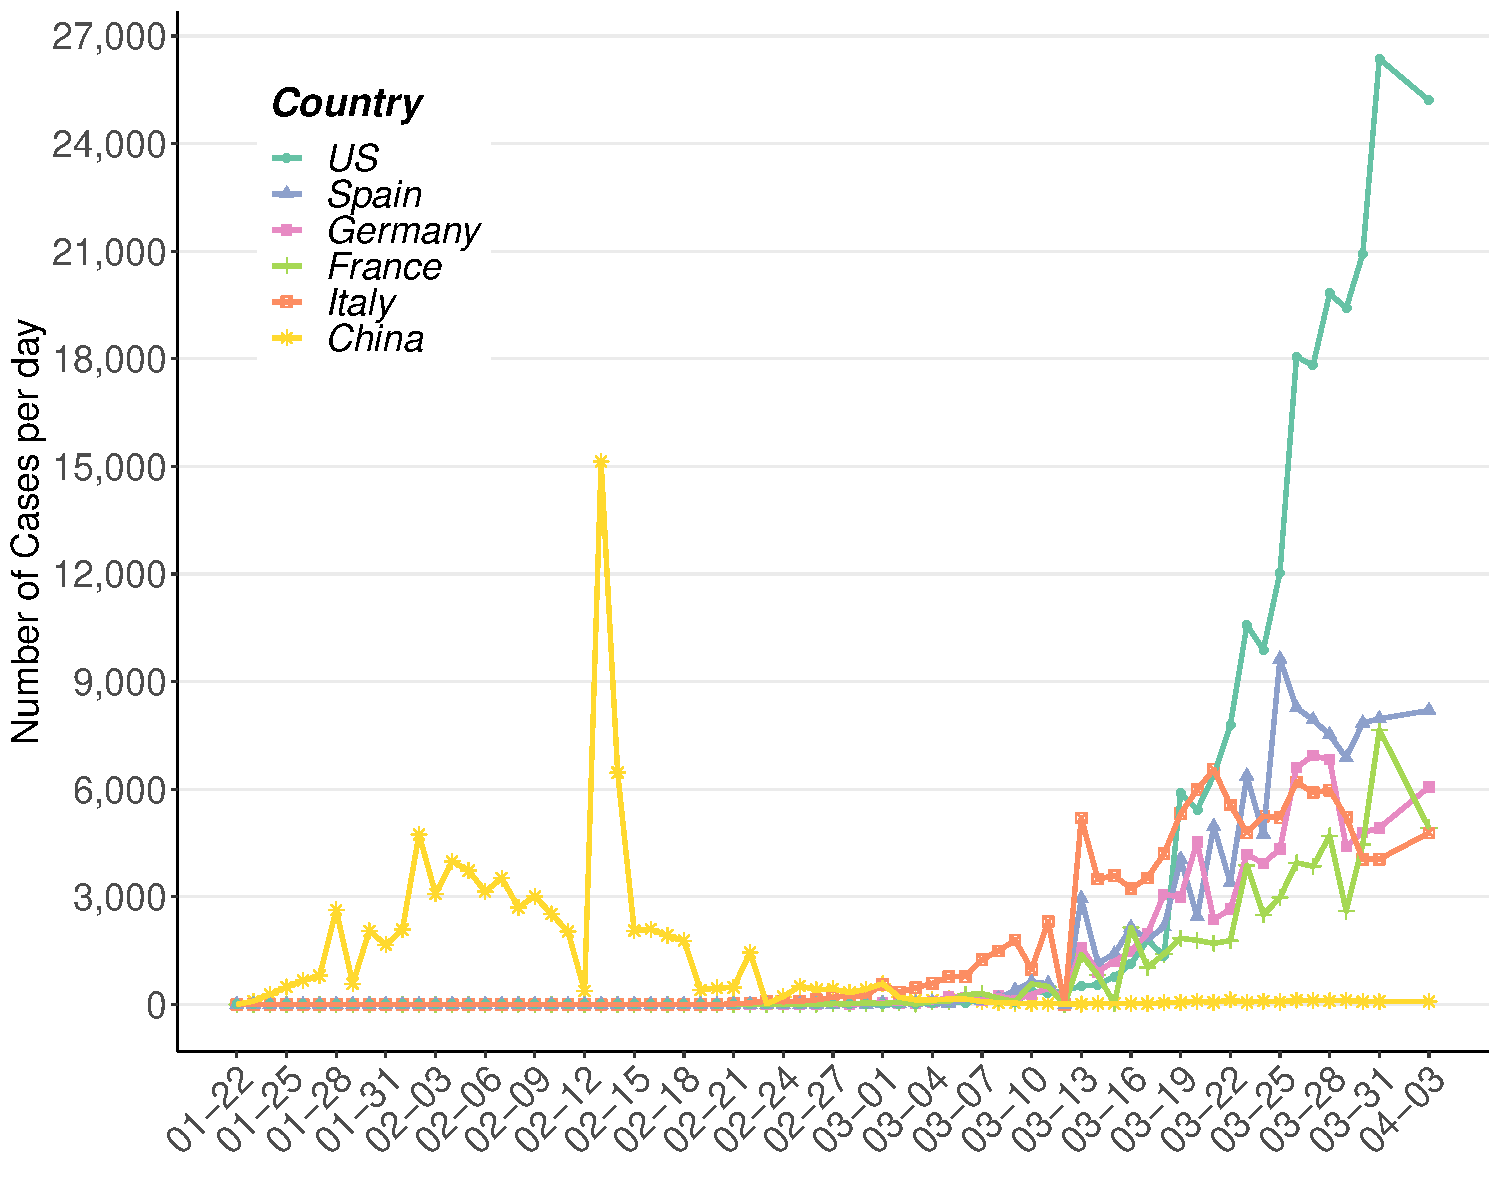
\includegraphics[]{./input/table_plot/covid3.pdf}
\caption{日新增确诊病例国家趋势图\\(中国及其他前五位国家)}
\label{}
\end{minipage}
\quad
\begin{minipage}[b]{0.45\linewidth}
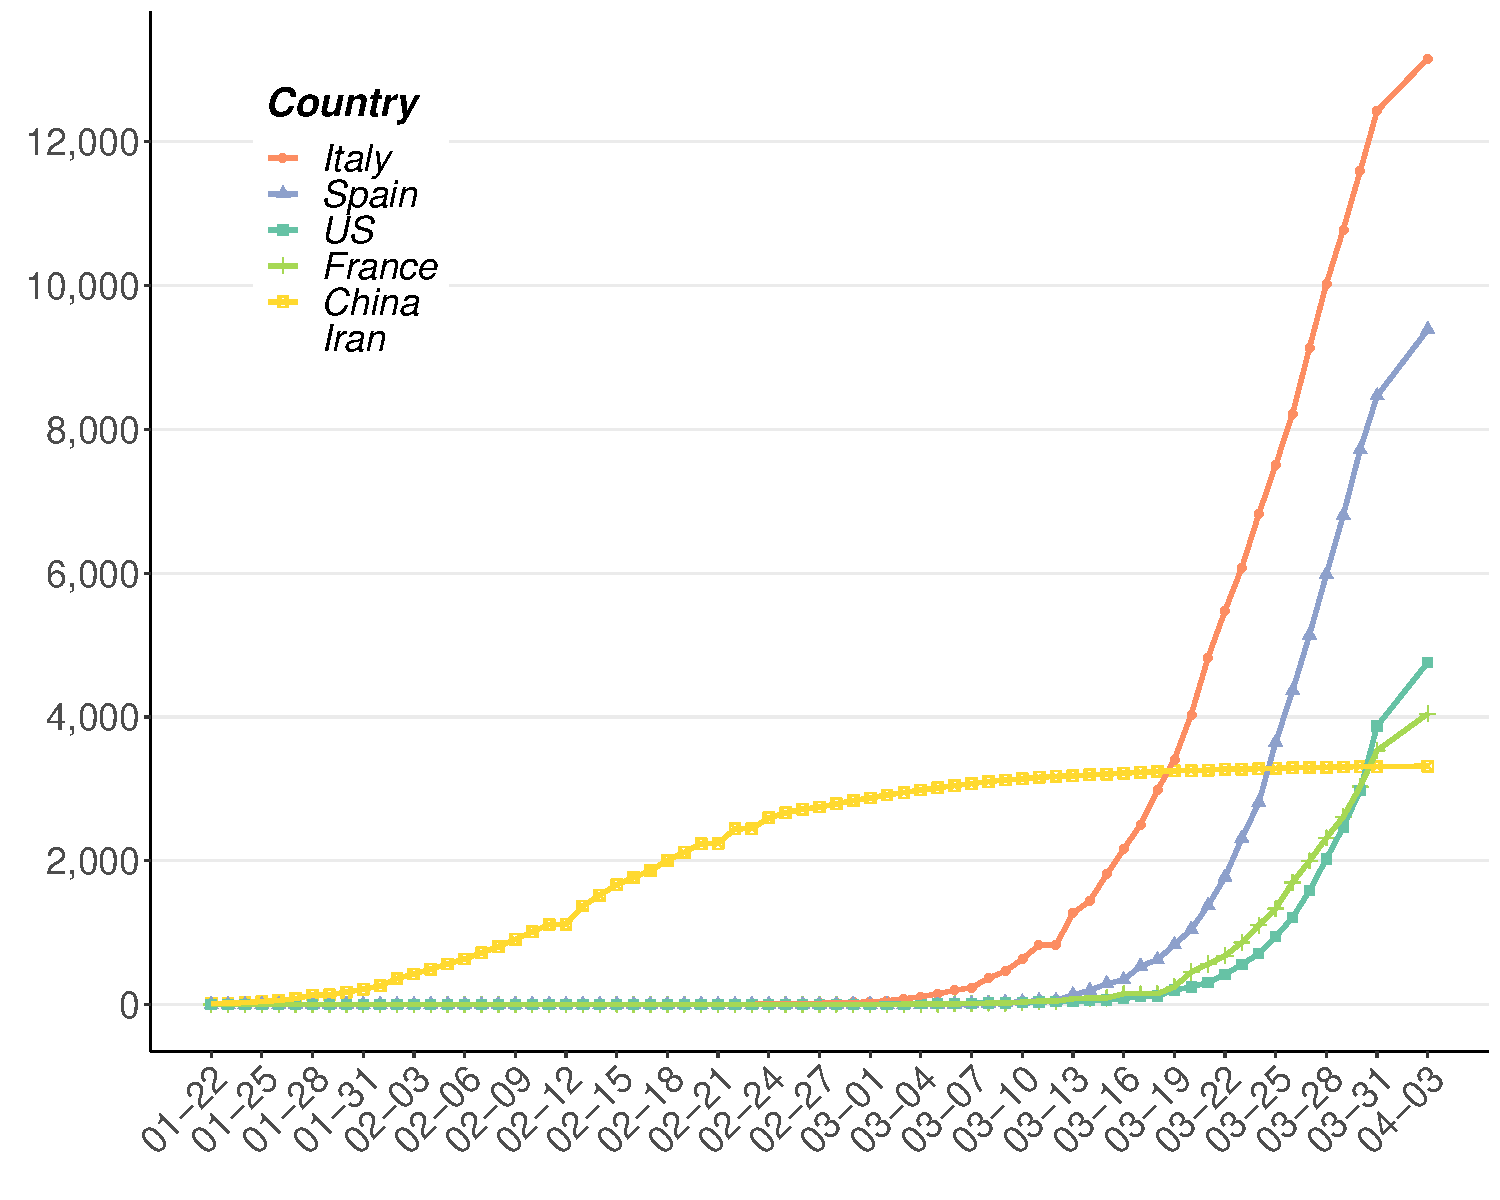
\includegraphics[]{./input/table_plot/covid4.pdf}
\caption{累计死亡病例国家趋势图\\(中国及其他前五位国家) }
\label{}
\end{minipage}
\end{figure}

\hypertarget{section-3}{%
\section{\texorpdfstring{\textcolor{glaucous}{二、美国疫情}}{}}\label{section-3}}

截至北京时间3月28日早6:00,美国共101,567例累计确诊病例,1,581例累计死亡病例。

\begin{figure}[H] 
\centering
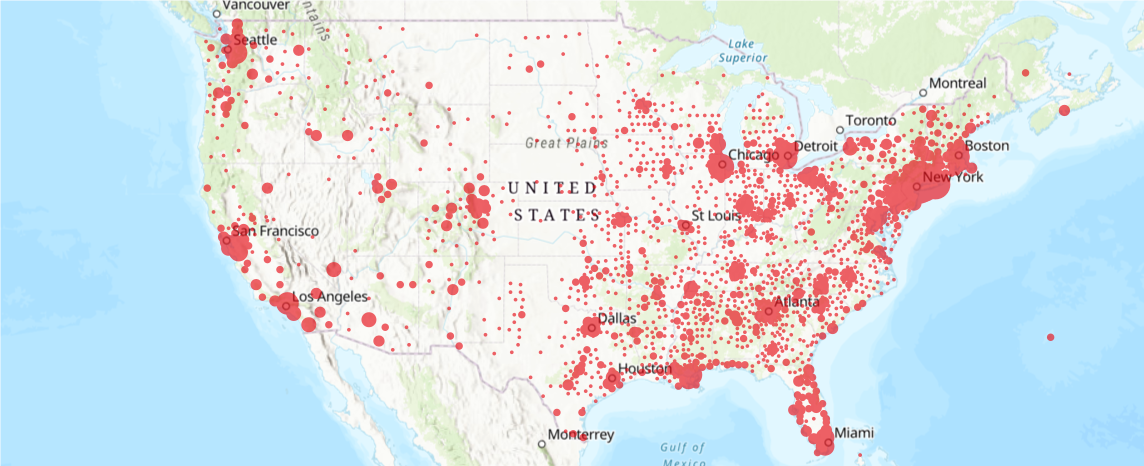
\includegraphics[]{./input/table_plot/covid5.png} %插入图片,[]中设置图片大小,{}中是图片文件名
\caption{美国本土疫情分布图 (Map of Cumulative Confirmed COVID-19 Cases in Contiguous U.S.)} %最终文档中希望显示的图片标题
\label{} %用于文内引用的标签
\end{figure}

\begin{minipage}{\textwidth}
        \begin{minipage}[H]{0.5\textwidth}
        \centering
           \begin{tabular}{@{}llll@{}}
           \toprule
              & 国家/州名         & 累计确诊  & 粗发病率 \\ \midrule
           1  & New York      & 83948 & 432  \\
           2  & New Jersey    & 22255 & 251  \\
           3  & California    & 9399  & 24   \\
           4  & Michigan      & 9315  & 93   \\
           5  & Massachusetts & 7738  & 111  \\
           6  & Illinois      & 6980  & 55   \\
           7  & Florida       & 6956  & 32   \\
           8  & Louisiana     & 6424  & 138  \\
           9  & Pennsylvania  & 6009  & 47   \\
           10 & Washington    & 5608  & 74   \\ \bottomrule
           \end{tabular}
            \makeatletter\def\@captype{table}\makeatother\caption{美国累计确诊前十位州}
        \end{minipage}
        \begin{minipage}[H]{0.5\textwidth}
        \centering
           \begin{tabular}{@{}llll@{}}
          \toprule
             & 国家/州名         & 当⽇新增 & 全美⽐率\% \\ \midrule
          1  & New York      & 8115 & 32     \\
          2  & New Jersey    & 3559 & 14     \\
          3  & Michigan      & 1700 & 7      \\
          4  & California    & 1189 & 5      \\
          5  & Louisiana     & 1187 & 5      \\
          6  & Massachusetts & 1118 & 4      \\
          7  & Pennsylvania  & 1046 & 4      \\
          8  & Illinois      & 986  & 4      \\
          9  & Georgia       & 709  & 3      \\
          10 & Texas         & 546  & 2      \\ \bottomrule
          \end{tabular}
      \makeatletter\def\@captype{table}\makeatother\caption{美国新增确诊前十位州}
    \end{minipage}
\end{minipage}

\begin{figure}[H]
\centering
\begin{minipage}[b]{0.45\linewidth}
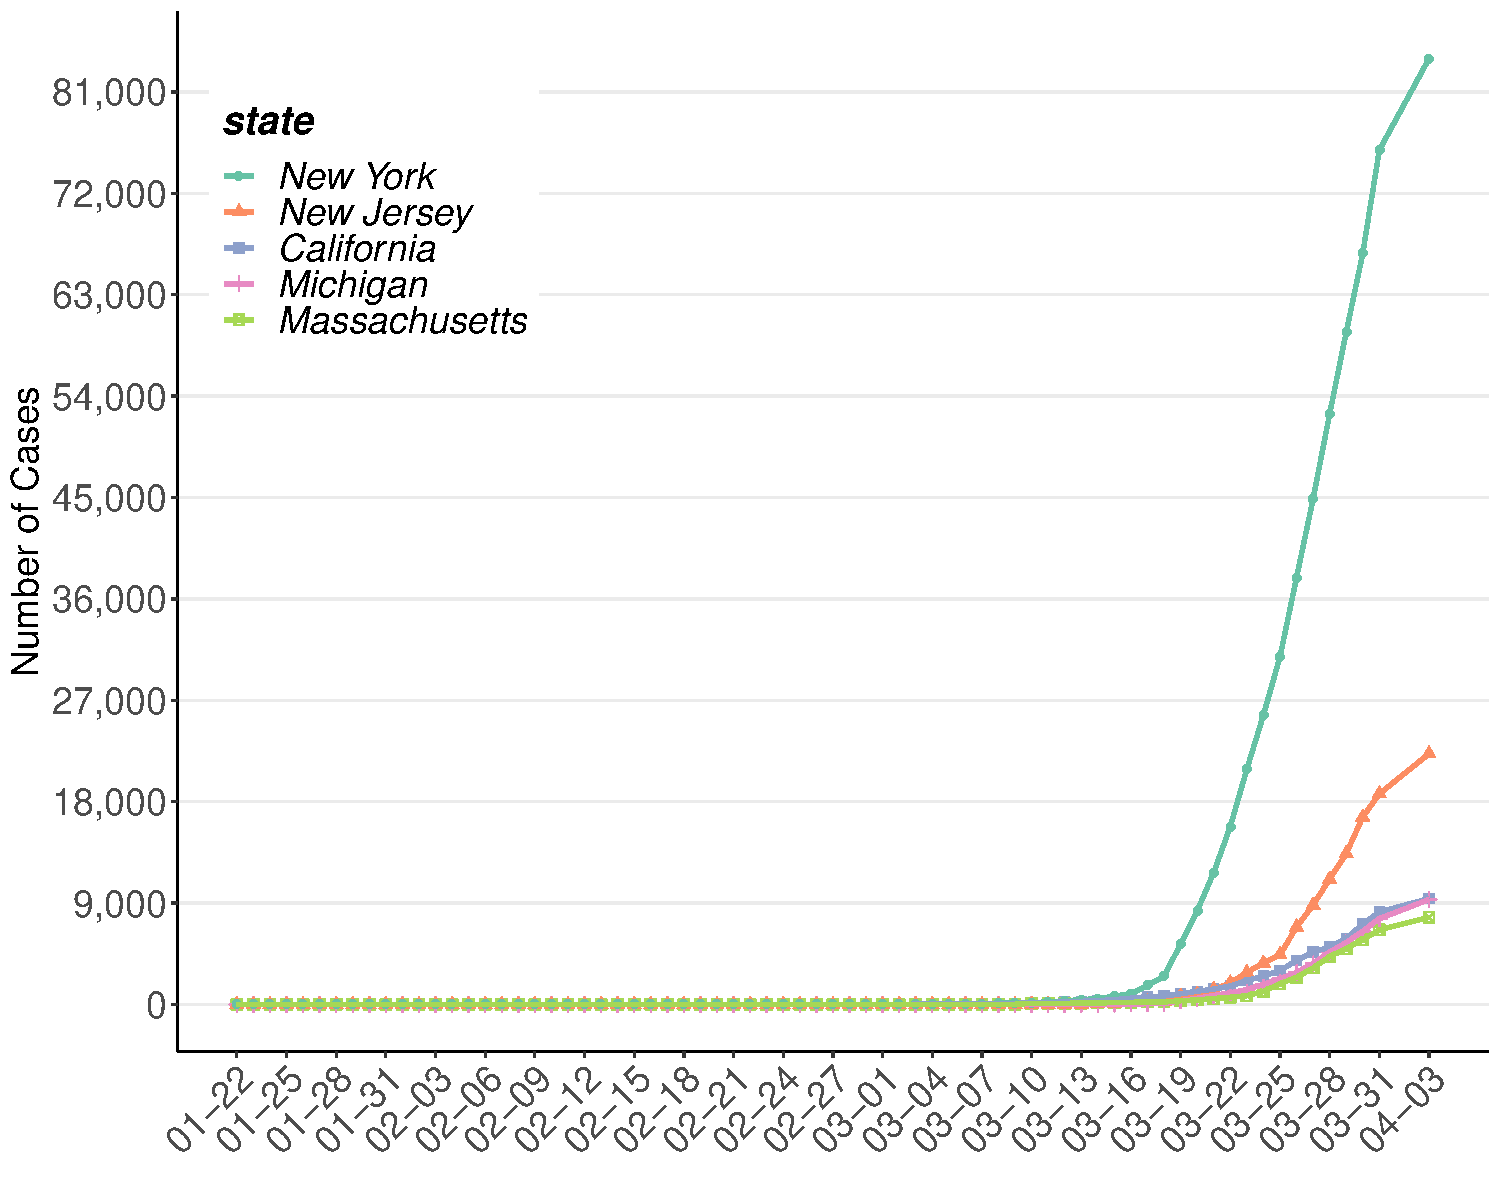
\includegraphics[]{./input/table_plot/covid6.pdf}
\caption{美国累计确诊前五位州趋势图}
\label{}
\end{minipage}
\quad
\begin{minipage}[b]{0.45\linewidth}
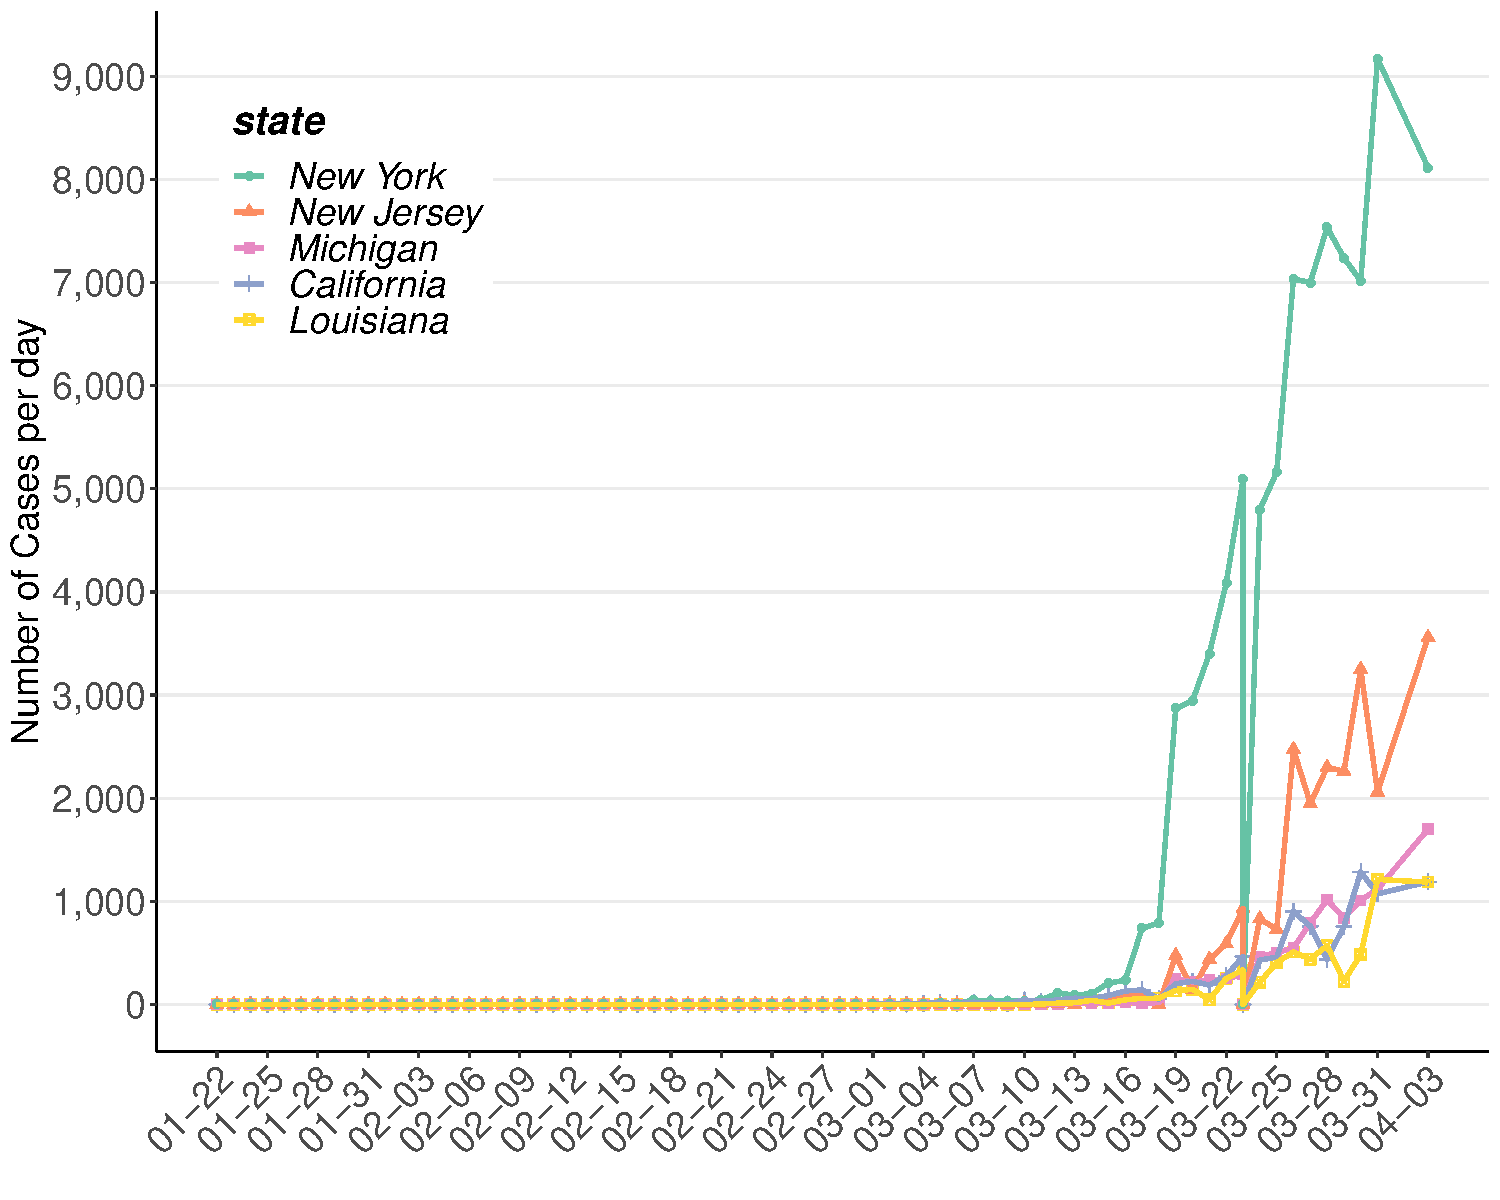
\includegraphics[]{./input/table_plot/covid7.pdf}
\caption{美国⽇新增确诊前五位州趋势图}
\label{}
\end{minipage}
\end{figure}

截至北京时间3月28日早6:00,美国共101,567例累计确诊病例,1,581例累计死亡病例。

\begin{table}[H]
   \centering
   \begin{threeparttable}[b]
   \resizebox{0.9\textwidth}{!}{%
      \begin{tabular}{p{.5cm}p{3.5cm}p{2.5cm}p{2.5cm}p{2cm}}
\toprule
   & 国家/州名         & 累计阳性病例 & 累计检测人数 & 阳性率\% \\ \midrule
1  & New York      & 1941   & 2.3    &       \\
2  & New Jersey    & 355    & 1.6    &       \\
3  & Michigan      & 335    & 3.6    &       \\
4  & Louisiana     & 273    & 4.2    &       \\
5  & Washington    & 234    & 4.2    &       \\
6  & California    & 199    & 2.1    &       \\
7  & Illinois      & 141    & 2      &       \\
8  & Georgia       & 139    & 3      &       \\
9  & Massachusetts & 122    & 1.6    &       \\
10 & Florida       & 87     & 1.3    &       \\ \bottomrule
\end{tabular}%
      }
      \begin{tablenotes}
     \item[*]北马利安纳群岛(MP)尚未大范围检测
   \end{tablenotes}
  \end{threeparttable}
   \caption{美国累计阳性率前十位州}
\end{table}

\begin{figure}
    \begin{minipage}[H]{0.5\linewidth}
    \centering
        \begin{tabular}{@{}lllll@{}}
        \toprule
           & 国家/州名 & 累计死亡⼈数 & 病死率\%  &      \\ \midrule
        1  & MI    & 10791  & 22684  & 0.48 \\
        2  & NJ    & 25590  & 59110  & 0.43 \\
        3  & OK    & 879    & 2144   & 0.41 \\
        4  & NY    & 92381  & 238965 & 0.39 \\
        5  & MP    & 8      & 21     & 0.38 \\
        6  & CA    & 9191   & 33000  & 0.28 \\
        7  & GA    & 5348   & 22957  & 0.23 \\
        8  & SC    & 1554   & 6995   & 0.22 \\
        9  & CT    & 3824   & 18300  & 0.21 \\
        10 & MS    & 1177   & 5930   & 0.2  \\ \bottomrule
        \end{tabular}
        \makeatletter\def\@captype{table}\makeatother\caption{美国累计死亡前十位州}
    \end{minipage}%
    \begin{minipage}[H]{0.5\linewidth}
    \centering
    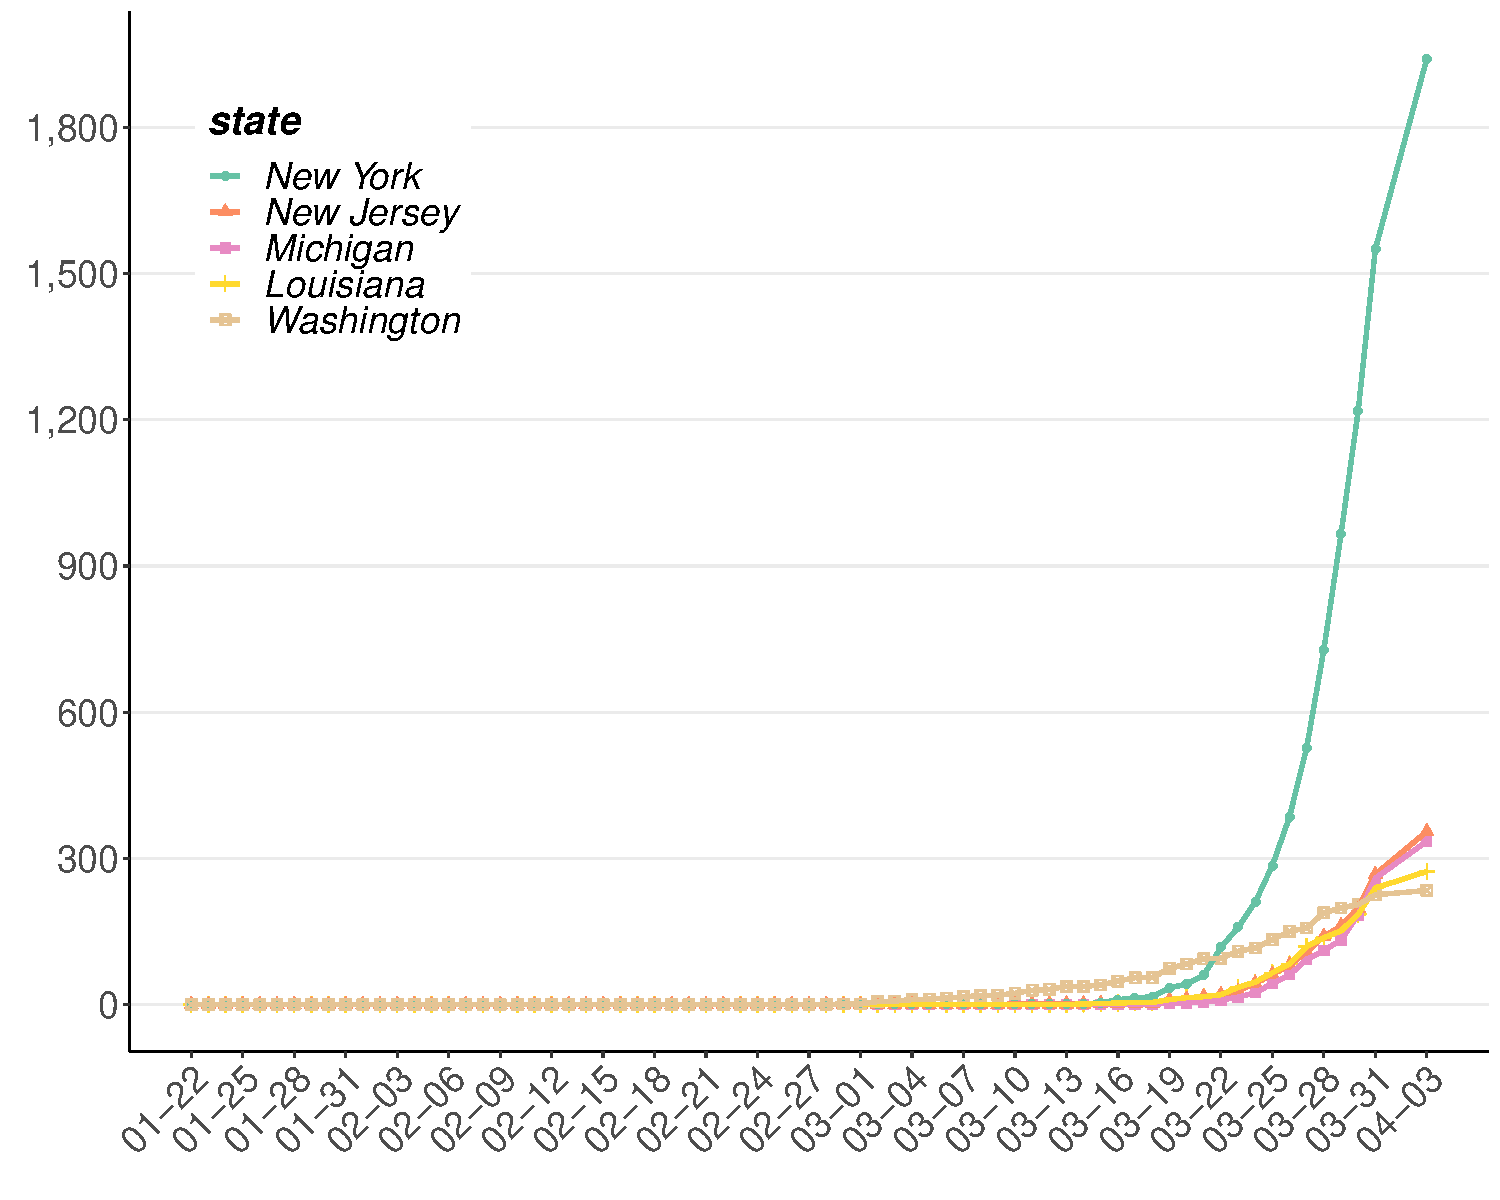
\includegraphics[]{./input/table_plot/covid8.pdf}
    \caption{美国累计死亡前五位州趋势图}
    \end{minipage}
\end{figure}

\begin{verbatim}
                    主编:马晶                  副主编:薛成海 仁晖 何鸿恺
                    执行责任编辑:史珂玮 王冠    新闻组:张宁 张心其
                    可视化组:霍舒同 张立达      数据分析:杜兆慧
                    感谢所有为日报作出贡献的志愿者:李忠锦 慕帼眉 李祎杰
\end{verbatim}

\end{document}
